\documentclass[11pt]{article}

\usepackage[margin=1.0in]{geometry}
%\linespread{1.5}
\usepackage{graphicx}
\usepackage{amsmath}
\usepackage{cite}

% definition of \customlabel, which is used to label supplementary figures and tables
\makeatletter
\newcommand{\customlabel}[2]{%
\protected@write \@auxout {}{\string \newlabel {#1}{{#2}{\thepage}{}{}{}}}}
\makeatother



\renewcommand{\bottomfraction}{.9}
\renewcommand{\topfraction}{.9}
\renewcommand{\textfraction}{0.1}
\renewcommand{\floatpagefraction}{.9}


\begin{document}
\title{\textbf{The relationship between dN/dS and scaled selection coefficients}}
\author{Stephanie J. Spielman$^{1}$ and Claus O. Wilke$^{1}$}
\date{}

\maketitle
\noindent
Address:\\
$^1$Department of Integrative Biology, Center for Computational Biology and Bioinformatics, and Institute of Cellular and Molecular Biology.
The University of Texas at Austin, Austin, TX 78712, USA.\\

\bigskip
\noindent
$^*$Corresponding author\\
$\phantom{^*}$Email: ??????????\\

\bigskip
\noindent Keywords: mutation-selection-balance models, mechanistic codon models, $dN/dS$, scaled selection coefficients, natural selection, protein evolution, models of sequence evolution

\newpage
\begin{abstract}
Two models which investigate strength of selection in protein-coding sequences are mechanistic codon models and mutsel models. We have measures of dN/dS and amino acid/codon ``propensities", which correspond to equilibrium frequencies. Are they the same? Are they different? We don't know! But now we do. And they're the same. This approach is really nice because it allows us to uncover properties of these metrics previously unidentified, etc. We found that codon-level models and metrics do not play nicely with amino-acid level models, and we found some interesting behaviors of the M0 model. Our study represents a very useful strategy - benchmarking and investigating model behavior be examining the intersection/relationship between distinct approaches.
  
  we can gain insight into model behavior by comparing the extent to which distinct modeling frameworks relate, or do not relate, to each other.
  
  
  There are two primary conclusions to our study: 1. it allows us to understand the relationship between distinct modeling frameworks. 2. It allows us to uncover properties of methods which would otherwise be impossible.

\end{abstract}

\section*{Introduction}

Over the years, various methods have been used to calculate the strength of natural selection acting on protein-coding sequences. Traditionally, the focus has been on estimating the evolutionary rate ratio, $dN/dS$, the rate of nonsynonymous to synonymous substitution rates. This metric indicates how quickly a protein's constituent amino acids change, and is widely used to identify cases of positive, diversifying selection ($dN/dS > 1$) \cite{NielsenYang1998, Yangetal2000, KosakovskyPondFrost2005, Huelsenbecketal2006}. Following early counting methods for estimating $dN/dS$ (e.g. refs \cite{LWL85} and \cite{NG86}), mechanistic codon models, which assume an explicit Markov-process model of sequence evolution (see ref.~\cite{Anisimova2009} for a comprehensive review), have taken a leading role as the inference method of choice since their introduction in the 1990s \cite{GoldmanYang1994, MuseGaut1994, NielsenYang1998}. These models yield maximum likelihood estimates (MLEs) for the parameter $\omega$, which represents the quantity $dN/dS$, and have seen great success in the field of molecular evolution. 

A second class of models, known as mutation-selection-balance (MutSel) models, have emerged recently as a popular alternative to mechanistic codon models. The MutSel framework, couched firmly in population genetics theory, models the dynamic interplay between mutation and selection in a protein-coding sequence. MutSel models yield estimates of site-wise scaled selection coefficients, which indicate the extent to which natural selection favors, or disfavors, particular codons or amino acids at a given protein position. Although MutSel models were first introduced over 15 years ago \cite{HalpernBruno1998}, they have seen virtually no use due to their high computational expense. Recently, however, several computationally tractable model implementations have emerged \cite{RodrigueLartillot2014,Tamurietal2014}, allowing for the first time the potential for widespread use. 

Although both mechanistic codon models and MutSel models describe the same fundamental process of protein-coding sequence evolution along a phylogeny, it is largely unknown how these two classes of models relate to one another. In particular, as these inference methods have been developed independently, it remains an open question whether or not parameter estimates from one model are comparable to those of the other model. Whether $dN/dS$ values have any correspondence with scaled selection coefficients remains an open question. Therefore, while certain rhetorical arguments may be made in favor of using one method over another, there is currently no formalized, concrete rationale to guide researchers in their methodological choices. 

Here, we formalize the relationship between mechanistic codon and MutSel models by examining the extent to which their focal parameters, $dN/dS$ and scaled selection coefficients, yield overlapping information about the evolutionary process. To this end, we derive a mathematical relationship between these models' primary parameters, allowing us to precisely infer $dN/dS$ values from scaled selection coefficients. Using a simulation approach, we verify that these derived $dN/dS$ values correspond precisely to $\omega$ MLEs inferred using standard mechanistic codon models. 


\section*{Methods}

We simulated protein-coding sequences as a continuous-time Markov process \cite{Yang2006} according to the MutSel model proposed by \cite{HalpernBruno1998}. This model's instantaneous rate matrix $Q$ is given by 

\begin{equation}\label{eq:BHmatrix}
Q_{ij} = \left\{ \begin{array}{rl}
              f_{ij}\mu_{ij}\kappa               &\mbox{single nucleotide transition} \\
              f_{ij}\mu_{ij}                          &\mbox{single nucleotide transversion} \\
              0                                           &\mbox{multiple nucleotide changes} \\             
         \end{array} \right.,
\end{equation}. Here, $\mu_{ij}$ is the nucleotide mutation rate and $f_{ij}$, the fixation probability from codon $i$ to $j$, is defined as 
\begin{equation} f_{ij}  = \frac{2Ns_{ij}}{1 - e^{2Ns_{ij}}}, \end{equation} where the value $2N_es_{ij}$ represents the scaled selection coefficient for a mutation from codon $i$ to codon $j$\cite{HalpernBruno1998, YangNielsen2008}. As shown by \cite{HalpernBruno1998}, the fixation probability \begin{equation}f_{ij} \propto ln\bigg{(}\frac{\pi_j\mu_{ij}}{\pi_i\mu_{ji}}\bigg{)}\bigg{/}\bigg{(}1 - \frac{\pi_i\mu_{ji}}{\pi_j\mu_{ij}}\bigg{)}.\end{equation} In this approximation, $\pi_i$ is the steady-state, or equilibrium, frequency of codon $i$. Importantly, these equilibrium frequency values are those which result from the joint effects of both mutation and selection. 

  
All alignments presented here were simulated along a 4-taxon phylogeny, beginning with a root sequence selected using steady-state codon frequencies. Unless otherwise stated, all simulated alignments contained 500,000 codon positions. A single evolutionary model was applied to all positions in the simulated sequences. While this lack of site-wise heterogeneity is unrealistic for real sequence evolution, it allows us to verify our derived relationship between equilibrium codon frequencies and $dN/dS$ with a sufficiently sized data set.


To demonstrate the relationship between $dN/dS$ and scaled selection coefficients, we simulated 100 sequences in which all synonymous codons have equal fitness (no codon bias), and 100 alignments in which synonymous codons featured different equilibrium frequencies (codon bias). For both sets of simulations, we assumed symmetric nucleotide mutation rates of $\mu_{xy} = 10^{-6}$ and $\kappa \sim \mathcal{U} (1,6)$.
We generated relative amino acid scaled selection coefficients $S_a$ for each simulation, by fixing one coefficient to 0 and drawing the remaining 19 values from a normal distribution $\mathcal{N}(0,\sigma^2)$, where $\sigma^2 \sim \mathcal{U}(0,4)$. Here, $\sigma^2$ effectively represents the strength of natural selection; larger values of $\sigma^2$ will correspond to greater fitness differences among amino acids, and thus more selective pressure. Moreover, these $S_i$ values correspond to the relative amino acid fitness parameters as inferred by currently available MutSel inference methods \cite{RodrigueLartillot2014,Tamurietal2014}.
For simulations without codon bias, we directly assigned $S_a$ values to codons such that all synonymous codons had the same scaled selection coefficient, and thus the same fitness.  For simulations with codon bias, we randomly selected a preferred codon for each amino acid. We then assigned the preferred codon a selection coefficient of $S_a + \lambda$ and all non-preferred codons a selection coefficient of $S_a - \lambda$. For each codon bias simulation, we drew $\lambda$ from $\mathcal{U}(0,2)$.

Finally, we computed equilibrium frequencies for all codons according to a Boltzmann distribution,  
   \begin{equation}\label{eq:pi_i}
 \pi_i=\frac{e^{S_i}}{\sum_k e^{S_k}}, \end{equation}
  where the denominator runs over all sense codons. Equation \eqref{eq:pi_i} directly relates codon equilibrium frequencies and ... using theory developed by Sella and Hirsh \cite{SellaHirsh2005}
Moreover, according to theory developed by Sella and Hirsh \cite{SellaHirsh2005}, these equilibrium frequencies are directly related to scaled selection coefficients according to 

We calculated a global $dN/dS$ for each alignment using the mathematical framework outlined in \eqref{eq:pi_i}--\eqref{eq:dS} as well using standard maximum likelihood methods. Specifically, inferred $dN/dS$ using the M0 mechanistic codon model \cite{Yangetal2000}, as implemented in the HyPhy batch language \cite{KosakovskyPondetal2005}. The M0 models uses the GY94 instantaneous rate matrix \cite{GoldmanYang1994,NielsenYang1998}, which includes the primary parameters $\omega$, $\kappa$, and equilibrium codon frequencies. For simulations inferences, we inferred $\omega$ both by fixing $\kappa$ to its true value, and maintaining $\kappa$ as a free parameter of the model. We used the Fequal equilibrium codon frequency model parameterization, which assigns equal frequencies of $1/61$ to all sense codons \cite{Yang2006}. Codon frequency parameters, unlike the steady-state codon frequencies of the underlying evolutionary model, are meant to capture mutational biases, and these parameters should correspond to the equilibrium codon frequencies which would be expected in the absence of selection \cite{YN00}, and a symmetric mutation process would produce equal frequencies of $1/61$.


Additionally, we simulated alignments which made use of experimentally-determined amino acid fitness and mutation rate data. We used site-wise influenza nucleoprotein (NP) amino acid preferences from Bloom 2014 \cite{Bloom2014a} and nucleotide mutation rates for either NP \cite{Bloom2014a}, yeast \cite{Zhu2014}, or polio virus \cite{Acevedo2014}. Note that all of these experimental mutation rate matrices were asymmetric. We combined each the 498 amino acid preference distributions with each set of nucleotide mutation rates to determine a total of $493 \times 3 = 1494$ unique experimental evolutionary Markov models, using the approach in Bloom \cite{Bloom2014a}, wherein the Metropolis acceptance criterion \cite{Metropolis1953} was used to calculate amino acid fixation rates. We calculated each model's equilibrium, or steady-state, codon frequencies such that detailed balance $\pi_i\mu_ij = \pi_j\mu_ji$ and $\sum\pi_i = 1$, where the sum runs across all 61 sense codons, was satisfied. Finally, for each set of equilibrium codon frequencies, we simulated alignments according to equation \eqref{eq:BHmatrix}.

We inferred $\omega$ for the simulations which employed experimental data with 5 different M0 model parameterizations. All inferences considered $kappa$ a free parameter of the model, but 5 different equilibrium codon frequency parameterizations were used. First, we inferred $\omega$ using the Fequal \cite{Yang2006} parameterization, which assigns equal codon frequencies of $1/61$ each. Second, we inferred $\omega$ by specifying codon frequencies which would arise strictly from mutational processes in the absence of natural selection. We computed these codon frequency values using the same approach as we did in calculating the true steady-state codon frequencies, except instead of using the experimental amino acid preference data, we all amino acids the same preference value of 0.05, thus eliminating any amino-acid level fitness differences. We term this frequency parameterization ``Fnull." Finally, we used the common frequency estimators F3x4 \cite{MuseGaut1994}, CF3x4 \cite{Pond2010}, and F61 \cite{GoldmanYang1994}. As typical analyses consider model frequency parameters as protein-wide, not site-specific, parameters, we computed these parameter values by pooling, for each set of mutation rates, 
all 498 steady-state codon frequencies to derive average codon frequencies. This approach yielded three distinct sets of averaged codon frequencies, from which we directly calculated the parameters for F3x4, CF3x4, and F61.








\section*{Results}


\section*{Mathematical relationship between $dN/dS$ and scaled selection coefficients}


We describe here how to calculate $dN/dS$ from scaled selection coefficients. MutSel models assume that both population size and selection pressure, and hence scaled selection coefficients, are constant across a given phylogeny \cite{HalpernBruno1998,YangNielsen2009,Rodrigueetal2010,Tamurietal2014}. Therefore, it is possible to derive stationary equilibrium frequenies for all codons. These equilibrium codon frequencies result from the dynamic interplay between both mutational and selective pressures. In the presence of symmetric nucleotide mutation rates, e.g. where $\mu_{xy} = \mu_{yx}$, we can compute analytically precise values for codon equilibrium frequencies according to theory developed by Sella and Hirsh \cite{SellaHirsh2005}, \begin{equation} \pi_i=\frac{e^{S_i}}{\sum_k e^{S_k}}, \end{equation} where the sum in the denominator runs over all 61 sense codons, and $S_i$ corresponds to the scaled selection coefficient for codon $i$. Alternatively, if nucleotides mutation rates are asymmetric, equilibrium codon frequencies can be numerically calculated though detailed balance conditions, such that the relationships 
 $\pi_i\mu_{ij} = \pi_j\mu_{ji}$ and $\sum\pi_i = 1$ are satisfied.
 
Using these equilibrium codon frequencies $\pi_i$, we can write the fixation probability for a mutation from codon $i$ to codon $j$ as \cite{HalpernBruno1998,SellaHirsh2005}
\begin{equation}\label{eq:f_ij}
 f_{ij} = \frac{1-(\pi_i/\pi_j)^{1/N_e}}{1-\pi_i/\pi_j}
  \approx \frac{1}{N_e} \frac{\ln \pi_j - \ln \pi_i}{1-\pi_i/\pi_j}\,,
\end{equation}
where $N_e$ is the effective population size. Through this framework, we can calculate an evolutionary rate by summing over all substitution probabilities weighted by the frequency of the originating codon. Further, we can establish specific expressions for nonsynonymous and synonymous evolutionary rates, and then divide them in order to obtain a value for the evolutionary rate ratio $dN/dS$.

To begin, we can write the nonsynonymous rate $K_\text{N}$ as 
\begin{equation}\label{eq:KN}
  K_\text{N} = N_e \sum_i \sum_{j \in {\cal N}_i} \pi_i  f_{ij}\mu_{ij}\,,
\end{equation}
where ${\cal N}_i$ is the set of codons that are nonsynonymous to codon $i$ and differ from it by one nucleotide. To normalize $K_\text{N}$, we divide it by the number of nonsynonymous sites, which we calculate according to the mutational opportunity definition of a site \cite{GoldmanYang1994, Yang2006} as 
\begin{equation}\label{eq:LN}
  L_\text{N} = \sum_i \sum_{j \in {\cal N}_i} \pi_i \mu_{ij}\,, 
\end{equation} and thus we find that 
\begin{equation}\label{eq:dN}
  dN = \frac{K_\text{N}}{L_\text{N}}=\frac{ N_e \sum_i \sum_{j \in {\cal N}_i} \pi_i f_{ij} \mu_{ij} } {\sum_i \sum_{j \in {\cal N}_i} \pi_i \mu_{ij} }\,.
\end{equation}

Similarly, for $dS$, the synonymous evolutionary rate $K_\text{S}$ per synonymous site $L_\text{S}$, we find
\begin{equation}\label{eq:dS}
  dS = \frac{K_\text{S}}{L_\text{S}}=\frac{ N_e \sum_i \sum_{j \in {\cal S}_i} \pi_i f_{ij} \mu_{ij} } {\sum_i \sum_{j \in {\cal S}_i} \pi_i \mu_{ij} }\,,
\end{equation}
where ${\cal S}_i$ is the set of codons that are synonymous to codon $i$ and differ from it by one nucleotide substitution. The quantities $K_\text{S}$ and $L_\text{S}$ are defined as in Eqs.~\eqref{eq:KN} and \eqref{eq:LN} but summing over $j\in {\cal S}_i$ instead of $j\in {\cal N}_i$.

Equations \eqref{eq:f_ij}--\eqref{eq:dS} establish a connection between the equilibrium codon frequencies and the evolutionary rate ratio $dN/dS$. Moreover, we note that, if we make the dual assumptions that nucleotide mutation rates are symmetric and that all synonymous codons have equal fitness (e.g. synonymous mutations are neutral), the synonymous fixation rate $f_{ij}= 1/N_e$ \cite{CrowKimura1970}. Under this circumstance, the value for $dS$ reduces to 1.

\subsection*{$dN/dS$ can be accurately predicted from scaled selection coefficients}

To validate the mathematical relationship between stationary codon frequencies and $dN/dS$ described in equations \eqref{eq:f_ij}--\eqref{eq:dS}, we simulated protein-coding alignments according to a MutSel model \cite{HalpernBruno1998,SellaHirsh2005}. We simulated 100 alignments in which synonymous codons had equal fitness values, and 100 alignments with codon bias, e.g. where the fitness values, and hence equilibrium frequencies, differed among synonymous codons (see Methods for details). All simulations described in this subsection used a symmetric nucleotide rate matrix, with the transition-tranversion bias ratio $\kappa \sim \mathcal{U}(1,6)$. Given these symmetric mutation rates, the codon equilibrium frequencies in these 200 simulations are directly proportional to their fitnesses \cite{SellaHirsh2005}. For each alignment, we calculated $dN/dS$ using equations \eqref{eq:f_ij}--\eqref{eq:dS} as well as using the M0 mechanistic codon model \cite{NielsenYang1998}, as implemented in the HyPhy batch language \cite{KosakovskyPondetal2005}.

The relationship between $dN/dS$ measurements is shown in Figure~\ref{reg_conv}A (for simulations with no codon bias) and Figure~\ref{reg_conv}B (for simulations with codon bias). It is clear that $dN/dS$ values derived using codon frequencies agree nearly perfectly with those inferred using standard maximum likelihood methods, and frequency differences among synonymous codons do not influence this robust relationship. Additionally, in Figure~\ref{reg_conv}C, we demonstrate convergence of $dN/dS$ estimates as the size of the data set, represented by simulated alignment length, increases. Taken together, these results demonstrate that MutSel model parameters fully encapsulate information regarding $dN/dS$, and that the results from MutSel and mechanistic codon models are in complete agreement.

Moreover, the strength of selection pressure scales fairly well with $dN/dS$. Figure~\ref{stddev_dnds} displays the relationship between $dN/dS$ and the standard deviation, $\sigma^2$, of the distribution of amino acid selection coefficients. Higher values of $\sigma^2$ indicate larger fitness differences among amino acids, ultimately leading to stronger selection pressure acting on nonsynonymous substitutions. Figure~\ref{stddev_dnds} demonstrates that when fitness differences among amino acids are very high, $dN/dS$ takes on lower values, properly reflecting stronger purifying selection. As expected, this trend is more robust for alignments without codon bias (Figure~\ref{stddev_dnds}A, $r^2 = 0.83$) than for alignments with codon bias (Figure~\ref{stddev_dnds}B, $r^2 = 0.45$). This weakened relationship emerges from the fact that fitness differences among synonymous codons obscure the underlying amino acid fitness differences. Thus, while a significant negative correlation remains, the codon bias generates increased noise.

Importantly, Figure~\ref{stddev_dnds}A shows that, in the limiting case when $\sigma^2$ approaches 0, and thus amino acids have virtually the same fitness values, $dN/dS$ converges to a value of 1. This result properly reflects the case of neutral evolution. In fact, in \textbf{SI proof}, we prove that, when synonymous codons have equal fitness values, $dN/dS$ is necessarily always less than or equal to 1. This restriction does not, however, hold in the face of codon bias, which can readily yield $dN/dS$ values greater than 1 (Figures \ref{reg_conv}B and \ref{stddev_dnds}B), even though the protein sequence is evolving under equilibrium conditions. We discuss the implications of these findings in depth in \textit{Discussion}.







% OLD PARAGRAPH WHERE WE USED ENTROPY INSTEAD OF STDDEV - We can additionally examine the extent to which $dN/dS$ relates to the strength of natural selection. As we employed a symmetric mutation matrix in these simulations, the codon equilibrium frequencies correspond precisely to codon fitness values \cite{SellaHirsh2005,deVladar2011}. Therefore, the distribution of equilibrium codon frequencies in fact represents the strength of purifying selection; when selection is strong, relatively fewer codons will be selectively tolerated, and thus the frequency distribution will be narrow. To examine the relationship between $dN/dS$ and selective strength, we computed the Shannon entropy $H = - \sum_i\pi_{i}\ln \pi_{i}$, where the sum runs over all 61 sense codons, for each set of equilibrium codon frequencies. Here, lower entropies correspond to more stringent purifying selection. Note that the maximum value of $H=4.11$ is achieved when all codons have an equal frequency of $1/61$. Figure~\ref{entropy_dnds} demonstrates that $dN/dS$ scales excellently with codon entropy; as entropy increases, $dN/dS$ similarly increases, properly reflecting the decrease in selection pressure. Moreover, while this trend holds both with and without the presence of synonymous codon fitness differences, the relationship between codon entropy and $dN/dS$ is stronger for simulations without codon bias (Figure~\ref{entropy_dnds}A, $r^2 = 0.901$) than with codon bias (Figure~\ref{entropy_dnds}B, $r^2 = 0.493$). This difference emerges from the fact that simulations with codon bias featured frequency, and hence fitness, differences among synonymous codons, obscuring the overarching fitness differences among amino acids. Figure~\ref{entropy_dnds}A also shows that, as codon entropy approaches its maximum value of 4.11, $dN/dS$ approaches, but never exceeds, the value of 1. In fact, in \textbf{SI proof}, we prove that, when synonymous codons have equal equilibrium frequencies, $dN/dS$ is necessarily always less than or equal to 1. This restriction does not, however, hold in the face of codon bias, which can readily yield $dN/dS$ values greater than 1 (Figures \ref{reg_conv}B and \ref{entropy_dnds}B), even though the protein sequence is evolving according to a steady-state process. We discuss the implications of these findings in depth in \textit{Discussion}.







\subsection*{Using real data/ML doesn't work so well/Jesse Bloom is prolific}

Results reported in the previous subsection were obtained from fully-simulated equilibrium codon frequencies, along with symmetric mutation rates. The latter assumption may not be entirely realistic; indeed, mutational biases, in particular transitions from $C/G \rightarrow T/A$ are known to contribute to uneven nucleotide compositions in real genomes \cite{Hernandez2007,HershbergPetrov2010,Zhu2014,Acevedo2014}. Therefore, we performed additional simulations which made use of realistic amino acid fitness and nucleotide mutation parameters.  In particular, we used influenza nucleoprotein (NP) site-specific amino acid preference values, given by Bloom \cite{Bloom2014a}. These data consisted of experimentally-determined fitness values for each individual amino acid across all sites in NP, yielding 498 distinct amino acid propensity distributions. We combined these experimental fitness parameters with three sets of experimentally determined mutation rates, either for NP \cite{Bloom2014a}, yeast \cite{Zhu2014}, or polio virus \cite{Acevedo2014}. Importantly, while all of these mutation matrices is asymmetric, they feature differing degrees of asymmetry, with NP mutation rates being the most symmetric and polio mutation rates the most asymmetric. For each of the 498 amino acid fitness distributions, we calculated stationary codon frequencies $\pi_i$ under detailed balance conditions, using the approach in \cite{Bloom2014a,Bloom2014b}. 

For each resulting set equilibrium codon frequencies, we again computed $dN/dS$ using equations \eqref{eq:f_ij}--\eqref{eq:dS} and simulated alignments according to equation \eqref{eq:BHmatrix}. We inferred $\omega$ MLEs using the M0 mechanistic codon model  according to five different codon frequency model parameterizations. These parameterizations included Fequal \cite{Yang2006} and the common frequency estimators F3x4 \cite{MuseGaut1994}, CF3x4 \cite{Pond2010}, and F61 \cite{GoldmanYang1994}. The estimators F3x4 and CF3x4 approximate codon frequencies using positional nucleotide frequencies, and the F61 estimator simply uses an alignment's empirical codon frequencies. Additionally, we inferred $\omega$ using a fifth frequency parameterization which consisted of the codon frequencies that would arise strictly from mutational processes, in the absence of natural selection. As this specification is the intended purpose for this parameter, we term it Fnull.


Figure~\ref{nyp_bias_r2} shows the resulting relationships between $dN/dS$ and $\omega$ MLEs for each set of mutation rates (NP, yeast and polio), across M0 model codon frequency parameterizations (Figure~\ref{nyp_regressions} contains regression plots for all simulated data sets and frequency parameterizations). Figure~\ref{nyp_bias_r2}A displays the bias, or systematic deviation from a 1:1 relationship, between $dN/dS$ and $\omega$, and Figure~\ref{nyp_bias_r2}B displays $r^2$ values between $dN/dS$ and $\omega$. Note that a bias of 0 would indicate a perfect correlation between $dN/dS$ and $\omega$ MLEs.


We find that $\omega$ MLEs generally correlate extremely well with $dN/dS$ values, but the strengths of these correlations differ among codon frequency model parameterizations (Figure~\ref{nyp_bias_r2}B). Overall, the Fnull parameterization performs the best of all frequency specifications; Fnull features both the least amount of bias and extremely high correlations. The Fequal parameterization similarly yields relatively low levels of bias, but its $r^2$ values drop precipitously for simulations using the yeast and polio mutation rates. This trend highlights the expected result that increasing asymmetry in mutation rates render Fequal an incorrect parameterization, as asymmetric mutation rates generate substantial compositional bias that Fequal cannot accomodate. Finally, the frequency estimators F3x4, CF3x4, and F61 perform well, and produced comparable correlations to the Fnull specification, with only marginally more bias. The purpose of these frequency estimators is to approximate the codon frequencies in the absense of amino-acid level natural selection \cite{YN00,Yang2006} (i.e., the Fnull parameterization), and our results indicate that these estimators accomplish this objective fairly well. 

Importantly, there is a clear trend that as asymmetric in mutation rates increase, the correlation strength systematically decreases, even for the Fnull parameterization (Figure~\ref{nyp_bias_r2}B). Clearly, including codon frequency parameters in mechanistic codon models does dramatically improve $\omega$ inferences, as is evidenced by the marked improvements of F3x4, CF3x4, and F61 over Fequal. Even so, as the negative bias values in Figure~\ref{nyp_bias_r2}A demonstrate, the M0 model systematically underestimates $dN/dS$ in line with increasing mutation rate asymmetry. This result suggests that incoporating codon frequency parameters may not be the optimal way to incorporate information on nucleotide compositional bias. 

However, there is a noteworthy exception to the trend of $\omega$ underestimation; the F61 frequency parameterization actually overestimated $\omega$ for simulations which employed NP mutation rates. We attribute this result to the fact that the NP mutation rates were only minimally asymmetric, featuring an average $\mu_{xy}/\mu_{yx} = 1.04$. Moreover, when nucleotide mutation rates are symmetric, steady-state frequencies are controlled only by selection, as there is no opportunity to generate compositional bias through mutation \cite{SellaHirsh2005}. As the F61 estimator directly uses empirical codon frequencies, the resulting M0 codon frequency parameters contain information about selection. Therefore, selective pressures which should be incorporated in the $\omega$ parameter are inadvertently contained within the codon frequency parameters, leading the model infer the strength of selection to be weaker than it truly is and produce elevated $\omega$ MLEs. Although the $\omega$ overestimatation was relatively minimal in this particular example, it serves as an important illstrative example of the necessity to properly parameterize mechanistic codon models. If these models are parameterized improperly, the $\omega$ parameter will no longer accurately represent the $dN/dS$ evolutionary rate ratio.



\subsection*{Discussion}

% may be useful to mention that many frameworks for dnds inference have been put forth over the years, and they are known to give conflicting results. Our approach to dnds inference is markedly different from these approaches, as it rests on population genetics principles rather than merely counting sites.
% our derivation yields the same results as does the standard, most-assumed-correct mech codon model. But it is clear that it is difficult to parameterize these models properly, especially given issues with codon frequencies not exactly doing what you what them to do, and likely being biased by sequence length. 
% this approach does, however make the assumption that there are indeed equilibrium codon frequencies that may be used. If a protein is evolving according to non-equilibrium processes, then there are no eq codon freqs, so this method is moot.
% previous efforts comparing among dnds calc methods all suffer because they all basically follow the same approach, except for how to deal with sites. This is really the difference among them. Here, this problem is basically removed.


% things that our study does not account for - gc bias produced by bias gene conversion. this is likely a selective force that systematically generates compositional bias, but cannot necessarily be accounted for amino acid selection coefficients. In theory, mech codon models incorporate this info via their codon frequency parameters, but mutation-selection models have no such equivalent parameter. possible future efforts could incorporate biases that stem from biological mechanisms other than amino acids and nucleotides.


The oldest and most-widely used method to infer selection pressure in protein-coding genes calculates the evolutionary rate ratio of non-synonymous ($dN$) to synonymous ($dS$) substitution rates. In turn, $dN/dS$ is commonly used to identify proteins or protein sites that experience negative selection ($dN/dS<1$), evolve neutrally ($dN/dS\approx1$), or that experience positive, diversifying selection ($dN/dS>1$) \cite{NielsenYang1998,Yangetal2000, KosakovskyPondFrost2005}. By contrast, MutSel models estimate scaled selection coefficients for amino acids, \cite{HalpernBruno1998,YangNielsen2008,Rodrigueetal2010,Tamurietal2012,Tamurietal2014}, for codons \cite{YangNielsen2008}, or for both. Thus, while mechanistic codon models describe the how quickly a protein's constituent amino acids change, MutSel models calculate the strength of natural selection operating on the specific amino-acid changes.  

Until now, however, it has been an open question how these two modeling frameworks relate to one another. Some have argued that MutSel models, given their firm grounding in population genetics theory and attention to site-specific amino acid fitness differences, offer a more fine-grained approach to studying protein evolution than do mechanistic codon models \cite{HalpernBruno1998,Rodrigueetal2010}. Recent phylogenetic studies have also demonstrated that evolutionary models which explicitly consider amino acid fitness values offer dramatic improvements over mechanistic codon models, suggesting that MutSel models may more aptly represent the process of coding-sequence evolution \cite{Bloom2014a, Bloom2014b}. 

Here, we have derived a formal mathematical relationship between the quantities $dN/dS$ and scaled codon selection coefficients, the primary parameters of mechanistic codon and MutSel models, respectively. Through a simulation approach, we find that these two models are in full agreement, and that the value for $dN/dS$ can be precisely calculated from scaled selection coefficients. Furthermore, this relationship is robust to fitness differences among synonymous codons. However, we note that our implementation of codon bias explicitly assumed that selection alone, and not mutation, was the sole source of codon bias. This implementation might not be entirely biologically realistic, as both mutational and selective forces likely contribute to codon bias in real genomes \cite{Blumer1991, Duret2002, HershbergPetrov2008, PlotkinKudla2010}. However, the key finding that we present is that fitness differences among synonymous codons do not affect the robust mathematical equivalency between scaled selection coefficients and $dN/dS$. 

We have also proven that, when synonymous codons have equal fitnesses and mutation rates are symmetric, $dN/dS$ will always be less than 1. This restriction does not, however, apply when synonymous codons have different fitness values (Figures \ref{reg_conv}B and \ref{stddev_dnds}B). In fact, when selection induces codon bias, it is possible to have arbitrarily high $dN/dS$ values; in the most extreme case of codon bias, in which only a single codon per amino acid is selectively tolerated, the number of synonymous sites $L_\text{S} = 0$, and thus the value for $dN/dS$ approaches infinity. Given that all simulations here assumed an overarching regime of purifying selection, the finding that $dN/dS$ can still be greater than 1 might seem paradoxical. However, the logical argument that $dN/dS > 1$ represents positive selection assumes that synonymous substitutions are selectively neutral, an assumption which is violated when synonymous codons have different fitnesses. Thus, in theory, what is classically termed positive selection can result simply from strong synonymous fitness differences. Even so, it is unlikely that this possibility will strongly influence real analyses, as selection on synonymous codons has been shown to be relatively weak in most taxa. Experimental evidence in the Hsp90 protein, for instance, demonstrates that while, while there are some fitness differences among synonymous codons, these differences are exceedingly minimal relative to fitness differences among amino acids \cite{Hietpas2011,Hietpas2013}. However, it is possible that estimates of positive selection in species with high levels of codon bias, such as bacterial, \textit{Drosophila}, or certain mammalian species \cite{Duret2002, Chamaryetal2006, HershbergPetrov2008, PlotkinKudla2010}, may not be true cases of positive selection, but rather simply signals of strong codon bias.

That the $dN/dS$ values calculated using equations \eqref{eq:f_ij} - \eqref{eq:dS} agree precisely with $\omega$ estimates inferred from the M0 mechanisic codon model lends firm support for the validity of our $dN/dS$ calculations. It has been long-recognized that different $dN/dS$ inference methods yield different $dN/dS$ estimates, as do different parameterizations of maximum likelihood mechanistic codon models \cite{YN00,Yang2006,ZhangYu2006}. Previously proposed frameworks for calculating $dN/dS$ have broadly fallen into two camps: heuristic counting methods \cite{LWL85,NG86,Pamilo1993,Ina1995,YN00} and maximum likelihood methods \cite{GoldmanYang1994,MuseGaut1994,Yang2006,Anisimova2009}. Unlike these frameworks, the $dN/dS$ calculations we have proposed here are solidly grounded in population genetics theory. That $\omega$ MLEs broadly agree with our $dN/dS$ calculations lend robust support to the accuracy of these $dN/dS$ values, and indeed to the methodological accuracy of mechanistic codon models. We emphasize, however, that the $dN/dS$ calculations we have proposed are only suitable when the protein is evolving under steady-state conditions, or in other words when selective pressure remains constant over time.

However, while the relationship between $dN/dS$ values and $\omega$ MLEs was remarkably strong under symmetric nucleotide mutation rates, the relationship weakened somewhat when we introduced asymmetric nucleotide mutation rates. As our $dN/dS$ calculations explicitly consider nucleotide mutation rates, we contend that this weakened relationship resulted from incorrect maximum likelihood $dN/dS$ inferences. In particular, the weakened relationship very likely resulted from model misspecifications in the M0 equilibrium codon frequency parameters. Mechanistic codon models attempt to deal with mutation-induced nucleotide compostional bias through equilibrium codon frequency parameters \cite{Yang2006}. Unlike the equilibrium steady-state frequencies we have focused on throughout this paper, these frequency parameters are intended to represent the codon frequencies which would exist in the absence of amino-acid level selection, but from mutational or other biological processes, such as biased gene conversion, alone \cite{GoldmanYang1994,MuseGaut1994,YN00,Yang2006}. If this parameter performs its task correctly, we would expect that a codon frequency parameterization which used precisely the correct parameter values would produce $\omega$ MLEs which agreed precisely with $dN/dS$. We did just this when inferring $\omega$ on alignments simulated with asymmetric mutation rates through the frequency parameterization Fnull. This specification gave the precise codon frequencies which mutation alone would generate, in the absence of selection. While this frequency specification did perform relatively well, and dramatically outperformed a model with equal codon frequencies, M0 still systematically underestimated $dN/dS$; as asymmetry in mutation rates increased, M0 underestimated $\omega$ more and more, and the correlation between $dN/dS$ and $\omega$ decreased. We can be sure that this trend did result entirely from asymmetric mutation rates, and simply from nucleotide compositional biases. Indeed, our alignments simulated with symmetric mutation rates featured a wide array of GC-contents, ranging from 0.18-0.72. Given these alignments' symmetric mutation rates, natural seletion favoring particular codons alone generated all compositional biases in those data sets, and maximum likelihood methods inferred $\omega$ perfectly under the Fequal frequency parameterization. 

Taken together, these results strongly suggest that the mechanistic codon model's codon frequency parameters might not be adequate to accomodate compositional biases which result from forces other than amino-acid level selection. We therefore suggest that future work investigate the utility of novel parameters for mechanistic codon models which better account for asymmetry in the mutational process.

Moreover, we emphasize that improper model parameterizations lead to spurious $\omega$ MLEs which do not accurately represent $dN/dS$, but instead some meaningless quantity. If other model parameters (e.g. $\kappa$ or the equilibrium codon frequencies) are specified incorrectly or inadvertently contain information about amino-acid level natural selection, the resulting $\omega$ MLE will not represent the true $dN/dS$ evolutionary rate ratio. Only by ensuring that $\omega$ is the only model parameter which contains information about natural selection will it assuredly represent $dN/dS$. This finding calls into question the use of the F61 frequency estimator, which assigns codon frequency parameter values based on empirical codon frequencies. If, by chance, a given alignment's protein-coding sequences evolved under symmetric mutation rates, these empirical codon frequencies will contain substantial information regarding the strength of natural selection, ultimately leading to incorrect $dN/dS$ inferences. Therefore, we recommend that users employ either the F3x4 \cite{MuseGaut1994} or the CF3x4 \cite{Pond2010} frequency estimators in their analyses.%It is also possible that the high correlations recovered were because all other values were properly specified, like $\kappa$. However, for inferences where we allowed $\kappa$ to be a free parameter, we recovered $r^2 = 0.998$, still remarkably high.






In sum, we have garnered several important insights into the behavior of mechanistic codon models, the $dN/dS$ metric, and selection coefficients. These results were only made possible through establishing a formal mathematical relationship between distinct modeling frameworks. We believe that the approach presented in this paper represents a promising future avenue for methodological benchmarking. Typically, researchers assess the performance of a given inference framework through simulations which adhere to the underlying model's assumptions. However, this strategy can only confirm that inference methods are behaving as expected; it cannot confirm that the underlying model accurately represents the evolutionary process. Instead, we suggest an alternate approach to benchmark inference methods, and indeed evolutionary models: assessing the extent to which distinct models agree may serve as a novel, robust strategy to determine the accuracy of different modeling frameworks and reveal previously unrecognized model properties or biases.




% % % % % % % % % % NONEQUILIBRIUM AND POSITIVE SELECTION STUFF % % % % % % % % % % %
%This relationship holds only if the protein evolves accordingly to a strictly steady-state process, otherwise known as purifying selection. Alternatively, under non-equilibrium conditions, (e.g. positive selection, when $\omega > 1$), MutSel models are inherently unable to describe protein evolution. These findings have important implications for when the use of each model is justified; if positive selection has occurred along the protein's evolutionary trajectory, MutSel models will likely yield spurious results. This proof, however, only holds when mutation rates are symmetric and when synonymous codons have equal fitnesses. 
%Our results rest on the key assumption that the protein sequence is evolving under steady-state, or equilibrium, conditions. The assumption exactly recapitulates the population genetics theory behind MutSel models, which assume that selection coefficients remain constant over the phylogeny, and therefore the protein is evolving along a static fitness landscape \cite{HalpernBruno1998,YangNielsen2008,Rodrigueetal2010,Tamurietal2012}. 
%Positive, diversifying selection is assumed to occur when the protein sequence experiences strong selective pressure to change its constituent amino acids. Positive selection, therefore, necessarily implies that the protein does not evolve at equilibrium, but rather a shift in selective constraint caused new amino acids to be favored. 
%  $dN/dS$ is used as a hallmark identifier for the three natural selection paradigms of purifying selection ($dN/dS < 1$), neutral evolution ($dN/dS = 1$), and finally positive selection ($dN/dS > 1$). Our analysis revealed that this classical $dN/dS = 1$ threshold might not be universally applicable. Indeed, all simulations presented here relied on the protein evolving under a steady-state process, or in other words, along a static fitness landscape. In a system where selective pressures remain constant along the phylogeny time, we expect purifying selection to dominate, and thus we should to recover only $dN/dS$ values less than 1. However, this was demonstrably not the case in several simulations which incorporated synonymous codon frequency, or fitness, differences (Figures~\ref{reg_conv}B and \ref{entropy_dnds}B). While simulations without codon bias all yielded $dN/dS < 1$, many simulations that incorporated codon bias featured $dN/dS$ values well above 1, with a maximum $dN/dS = 1.82$. In fact, we prove in \textbf{SI proof} that, under general conditions of a symmetric mutation and equal synonymous codon frequencies, $dN/dS$ is necessarily always less than or equal to 1. This proof, however, does not extend to cases of synonymous fitness differences, in spite of the steady-state evolutionary process. 
%In proteins evolving under equilibrium, a fundamental assumption of MutSel models, the terms purifying and positive selection may not generally apply. Instead, we suggest that these terms be strictly reserved for the fitness effects of individual amino acid changes, rather than applying them as overall terms for the protein's evolutionary trajectory. Indeed, while it may easily be said that certain amino acid changes are acted on by pos or pur selection, the protein, or residue/position, itself is either evolving under equilibrium or non-equilibrium conditions. Equilibrium evolution can involve pur and pos, but the expectation is that, at the end of the day, it will average out to purifying selection since the fitness landscape is static. Everybody seems to be very imprecise about this. MutSel papers all state that an assumption is purifying selection, and then they go on to spend half the paper identifying instance of purifying vs. positive selection. This is a little bit ridiculous, semantically, so I'm writing something about how we need increased precision in our wording. Sella\&Hirsh theory enters this discussion very well, in that they contend that equilibrium evolution necessarily involves just as many adaptive as deleterious substitution events. Thus, equilibrium evolution cannot be confused with purifying selection, and positive selection does not always represent the introduction of a novel selection pressure.Maybe future work could get at distinguishing between positive selection when it arises the context of steady-state evolution vs when it is induced by a novel fitness landscape.





\clearpage
\newpage
\bibliographystyle{plos2009}
\bibliography{bibliography}	

\clearpage
\newpage	

\begin{figure*}[H]
\centerline{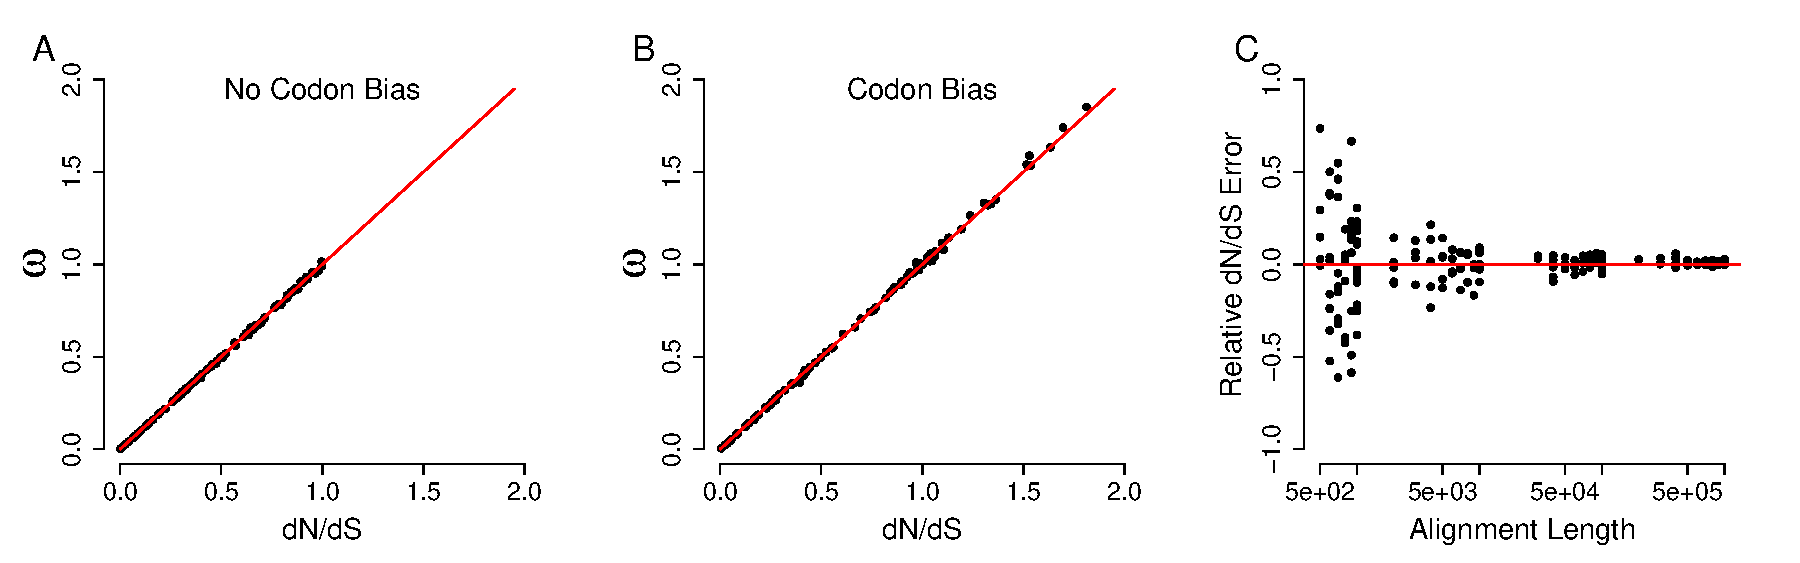
\includegraphics[width=6in]{figures/MainText/regression_convergence.pdf}}
\caption{\label{reg_conv} Relationship works exceedingly well. Left panel shows 100 points, each of which corresponds to single simulation. Note that here the ml inference is shown for equal codon frequency specs and kappa fixed to true value (a similar plot for free kappa is shown in suppfigs, but results are qualitatively identical.) Right panels shows convergence of omega values as data set size (represented as simulated alignment length) increases. The y-axis indicates relative error of the ML $dN/dS$ estimates, and the x-axis indicates sequence length on a log-scale. As the sequence length, or the data set size, increases, the two $dN/dS$ estimates converge to the same value. }
\end{figure*}


\bigskip
\begin{figure*}[H]
\centerline{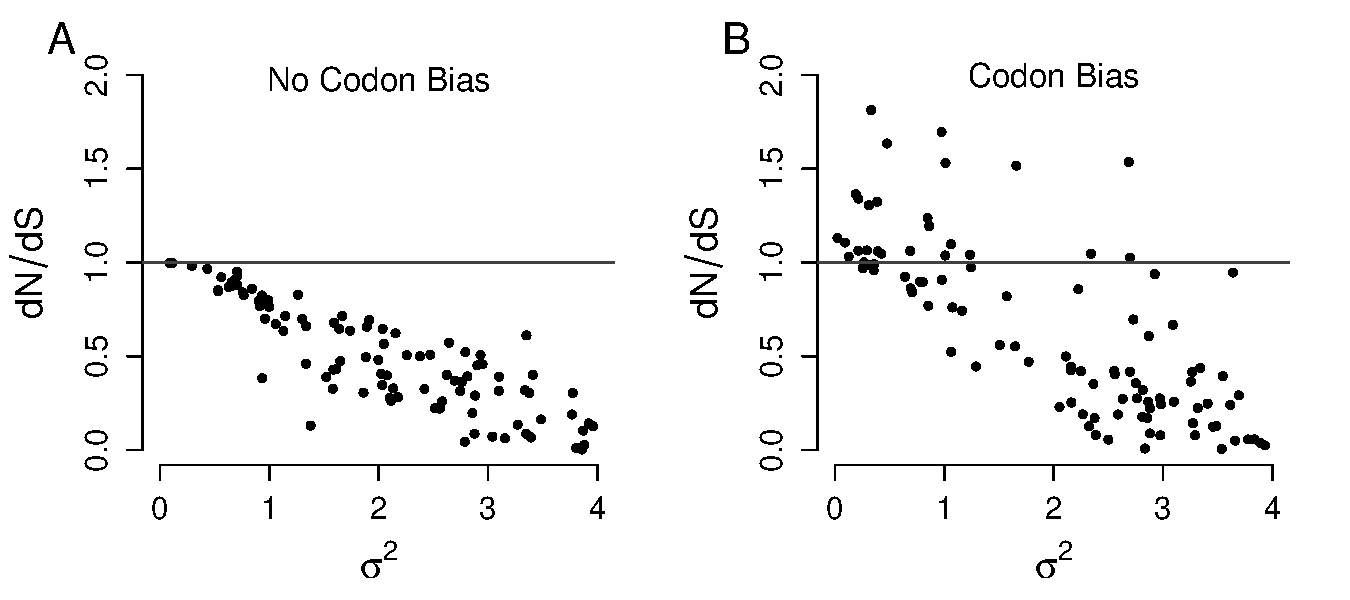
\includegraphics[width=4in]{figures/MainText/sd_vs_dnds.pdf}}
\caption{\label{stddev_dnds} strength of selection scales well with dnds but the strength of the relationship diminishes with codon bias as synonymous now have frequency differences, so dnds is less of a reliable indicator of selection strength.}
\end{figure*}


\bigskip
\begin{figure*}[H]
\centerline{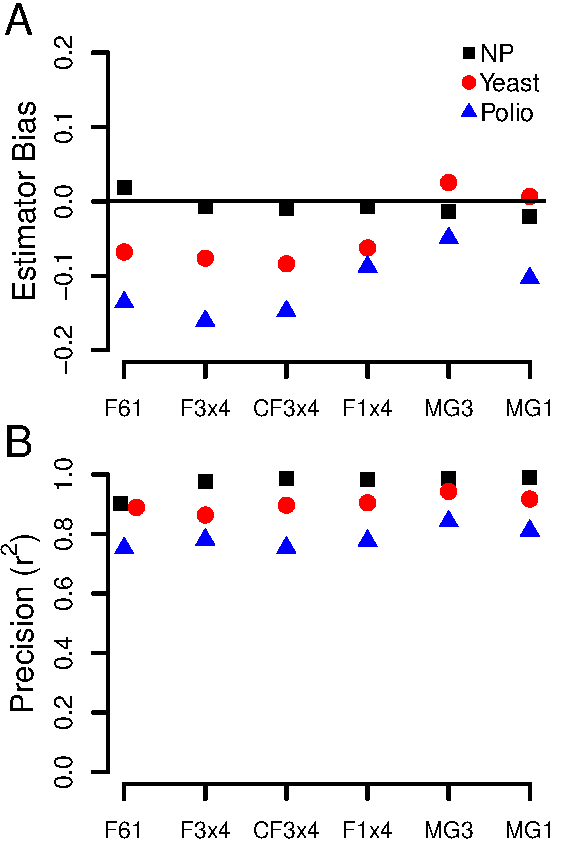
\includegraphics[width=6in]{figures/MainText/nyp_bias_r2.pdf}}
\caption{\label{nyp_bias_r2} Global outperform, obviously. Clear that the null is probably the best bet. The question is, how well to commonly used estimators approximate this null specification? Decently, but clearly F3x4 and CF3x4 do better than F61. Also, Fequal does reasonably well, but it gets noisy as the asymmetry in mutation rates grows.}
\end{figure*}

\clearpage
\newpage
\centerline{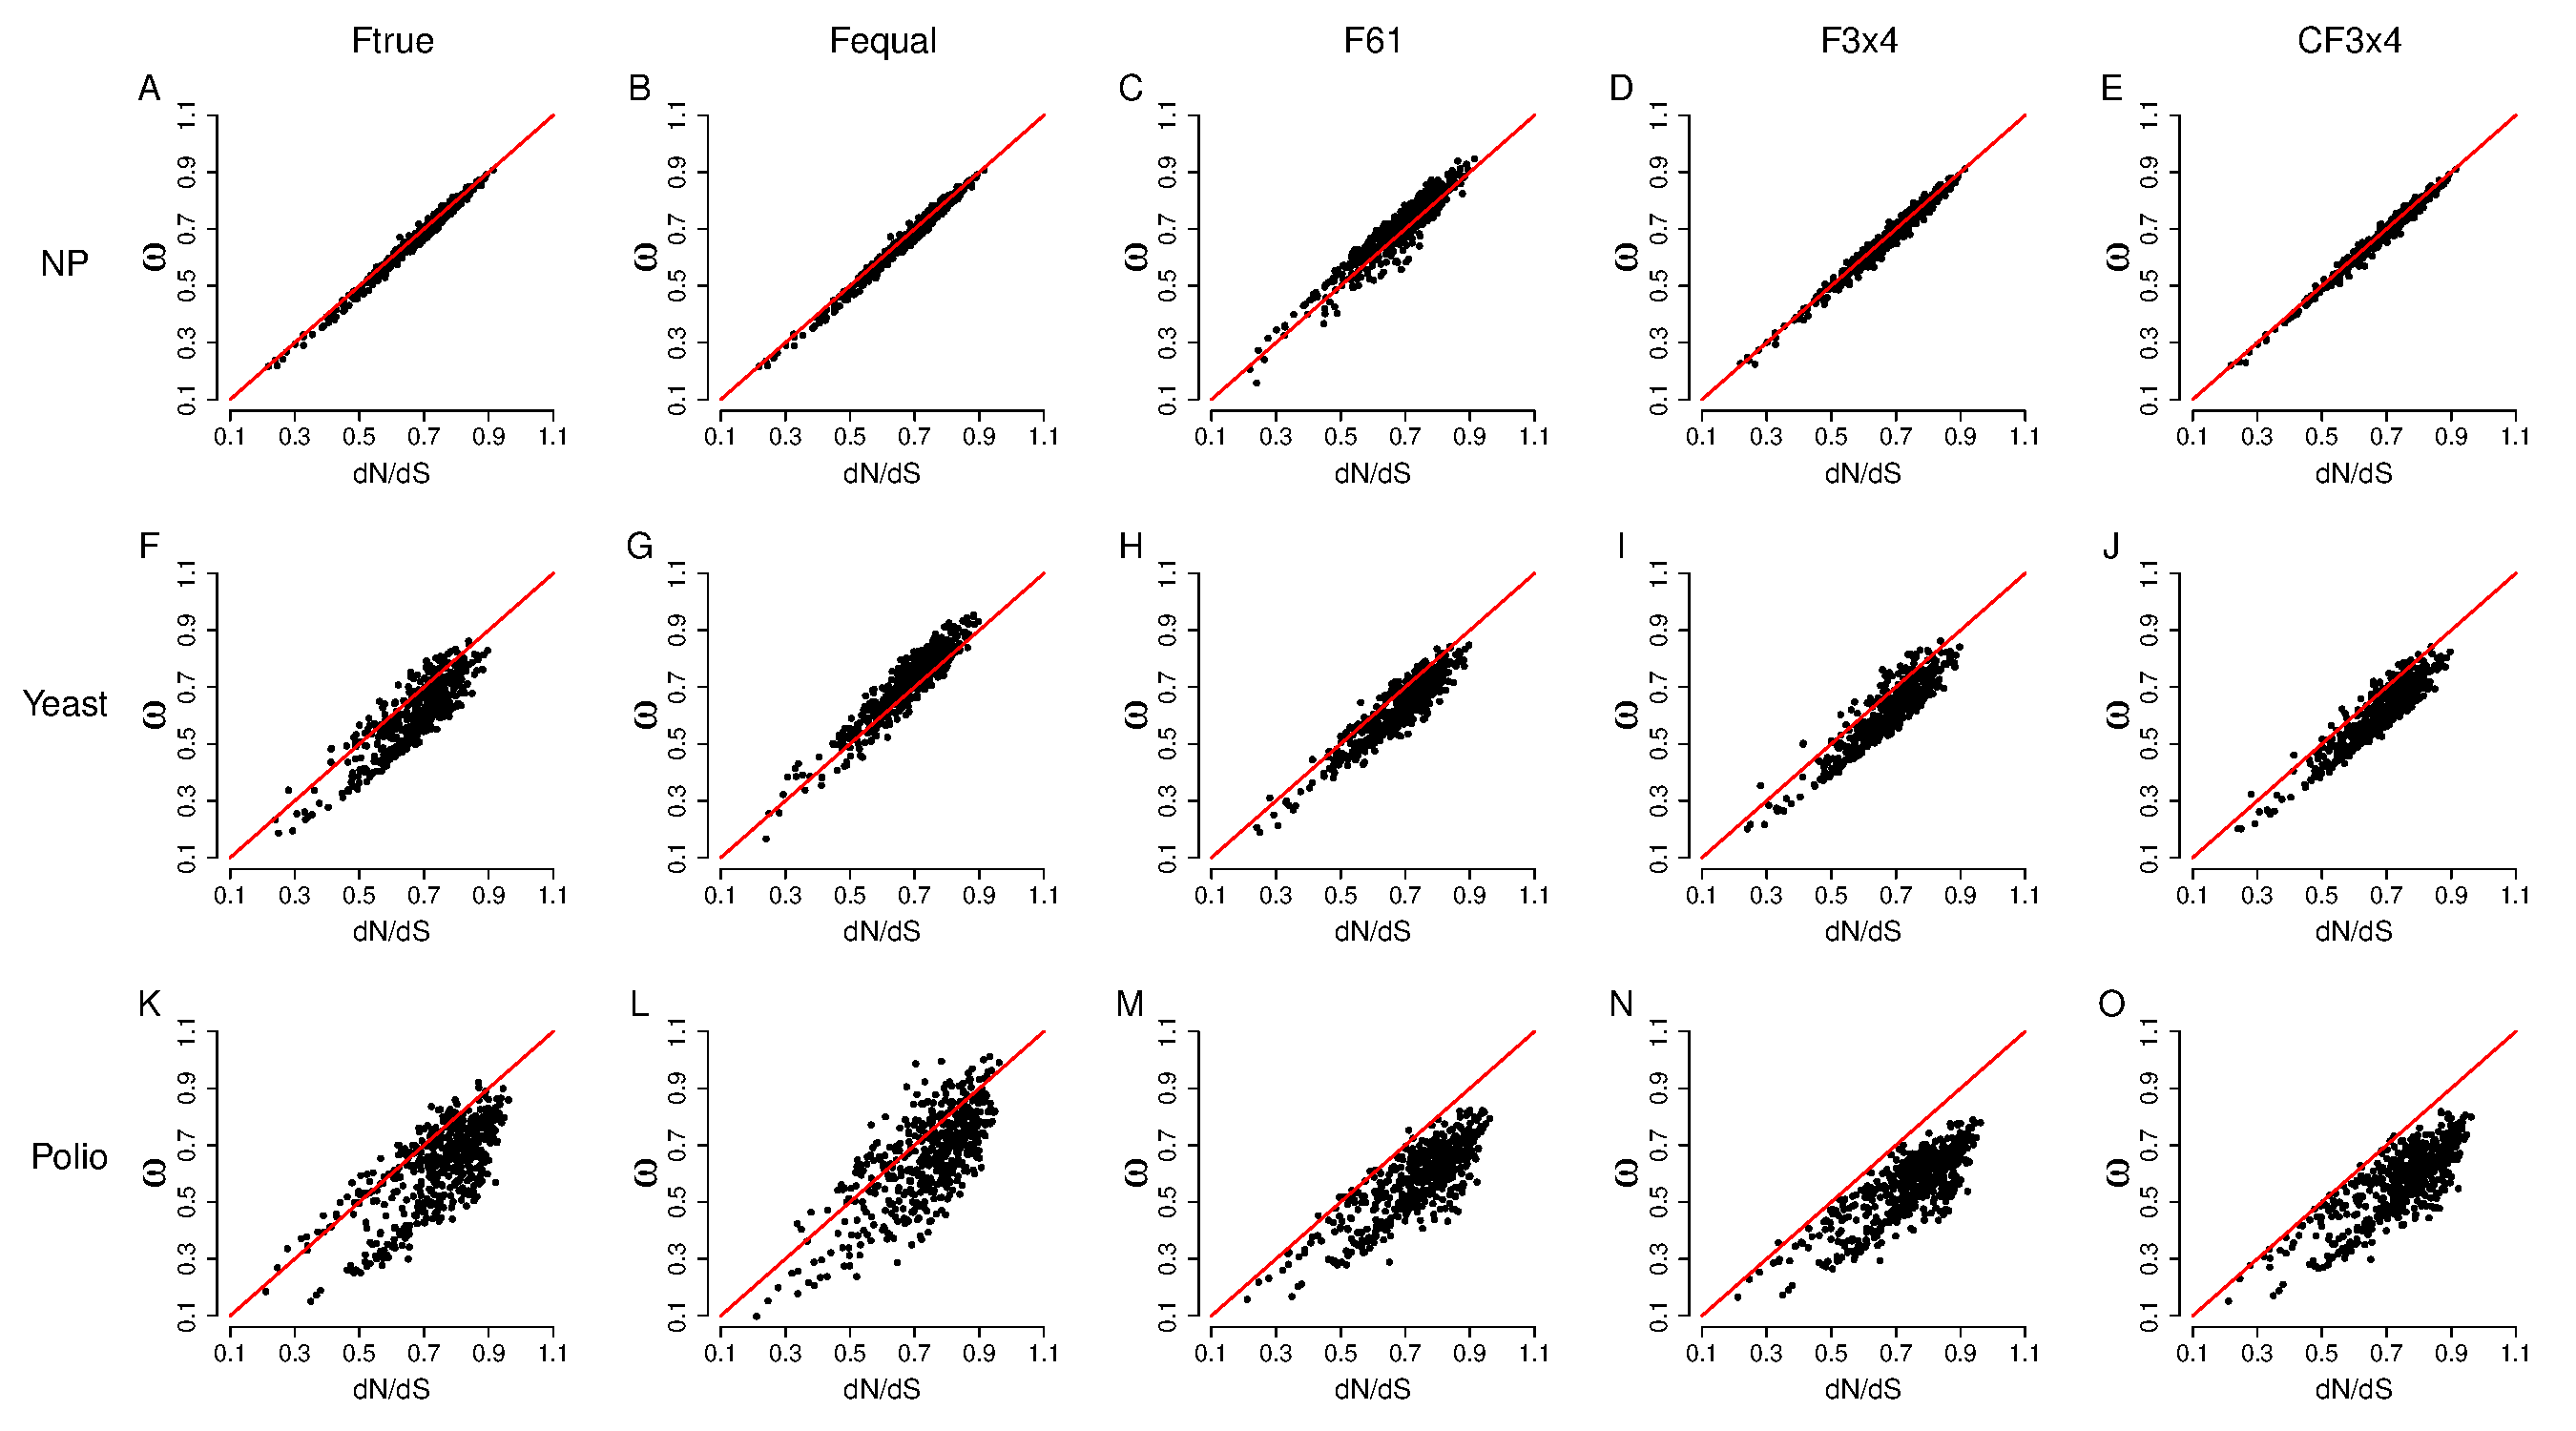
\includegraphics[width=8in]{figures/SI/nyp_fspecs_full.pdf}}
\noindent \textbf{Fig. S1} Omega regression for all ML parameterizations for the np, yeast, and polio mutation rates.
\customlabel{fig:nyp_regressions}{S1}




\end{document}

